\documentclass[12pt]{article}
\usepackage{graphicx}
\usepackage{float}
\usepackage{setspace}
\usepackage{geometry}
\usepackage[utf8]{inputenc}
\usepackage[T1]{fontenc}
\usepackage{amsmath}
\usepackage{amsfonts}
\usepackage{amssymb}
\usepackage{enumitem}
\usepackage{hyperref}
\usepackage{booktabs}
\usepackage{caption}
\usepackage{subcaption}
\usepackage{xcolor}
\geometry{margin=1in}

\title{Scientific Calculator with DevOps\\ \large Comprehensive Mini Project Report}
\author{}
\date{}

\begin{document}

% ============================
% Custom Title Page
% ============================
\begin{titlepage}
\centering

\textbf{\Large International Institute of Information Technology 
Bangalore}\\[0.5cm]

\textbf{\Large Software Production Engineering}\\
\textbf{CS 816}\\[1.2cm]

\rule{\linewidth}{1.5pt}\\[0.2cm]
\rule{\linewidth}{0.5pt}\\[0.5cm]
{\Huge \textbf{Mini Project Report}}\\[0.3cm]
{\LARGE \textbf{Scientific Calculator with DevOps}}\\[0.5cm]
\rule{\linewidth}{0.5pt}\\[0.1cm]
\rule{\linewidth}{1.5pt}\\[2cm]

\textbf{Shikhar Bhadreshkumar Mutta (MT2025114)}\\[2cm]

\href{https://github.com/shikhar-mutta/Scientific-Calculator-with-DevOps}{\texttt{Github Link}}\\
\href{https://hub.docker.com/repository/docker/shikhar68/scientific-calculator/general}{\texttt{Docker hub Link}}\\[1cm]



\textbf{\today}\\[3cm]

\includegraphics[width=0.25\textwidth]{imgs/IIITB_logo.png}\\[0.3cm]
% Uncomment and replace with actual logo if available
% \includegraphics[width=0.25\textwidth]{IIITB_logo1.png}\\[0.3cm]

\end{titlepage}

\tableofcontents
\newpage

\section{Introduction: What and Why of DevOps?}

\textbf{What is DevOps?}\\
DevOps is a set of cultural philosophies, practices, and tools that combines software development (Dev) and IT operations (Ops). It aims to shorten the systems development life cycle while delivering features, fixes, and updates frequently in close alignment with business objectives.
\vspace{0.3cm}

\textbf{Why DevOps?}\\
In the context of this scientific calculator project, manual compilation, testing, and deployment of the Java application are prone to human error and are highly time-consuming. Adopting DevOps methodologies automates these processes. A Continuous Integration and Continuous Deployment (CI/CD) pipeline ensures that every time a developer commits code to the repository, it is instantly built, rigorously tested against edge cases, smoothly containerized, and deployed to production servers without manual downtime.

\section{Tools Used}
The complete end-to-end automated pipeline relies on the following DevOps toolchain:
\begin{itemize}
    \item \textbf{Source Control Management:} GitHub
    \item \textbf{Build Tool:} Maven
    \item \textbf{Testing Framework:} JUnit
    \item \textbf{Continuous Integration:} Jenkins
    \item \textbf{Containerization:} Docker
    \item \textbf{Configuration Management:} Ansible
\end{itemize}

\begin{figure}[H]
\centering
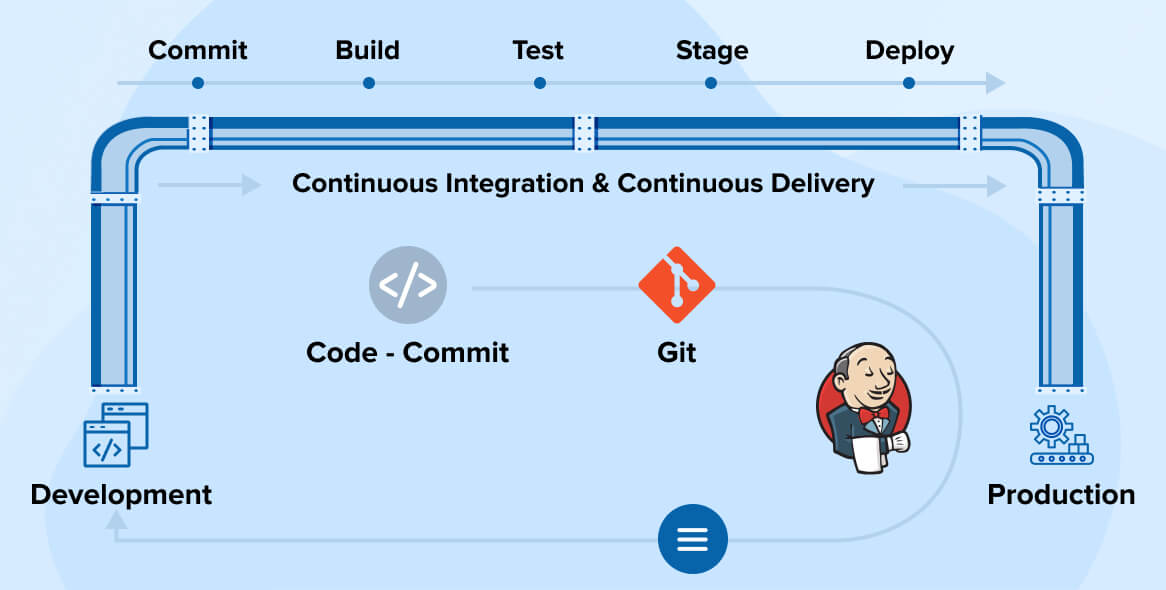
\includegraphics[width=0.8\textwidth]{imgs/CICD-w-Jenkins.jpg}
% \fbox{\rule{0pt}{2in}\rule{4in}{0pt}}
\caption{High-level architectural diagram of the CI/CD pipeline}
\end{figure}

\newpage

\section{Jenkinsfile --- Stage-by-Stage Explanation}

\begin{figure}[H]
\centering
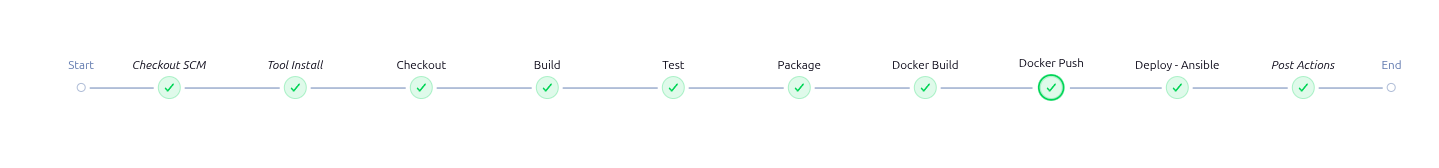
\includegraphics[width=\textwidth]{imgs/Jenkins Stages v1.png}
\caption{Jenkins Pipeline Stages}
\end{figure}

\subsection{Global Configuration}
\noindent
\begin{minipage}[t]{0.38\textwidth}
\captionsetup{type=figure}
\vspace{0pt}
\centering
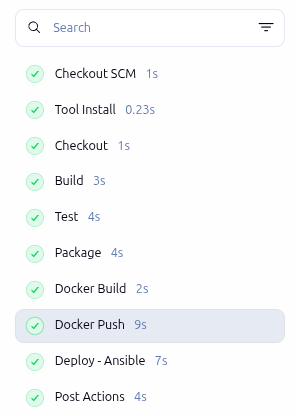
\includegraphics[width=\textwidth]{imgs/Time taken by stages.png}\\[-6pt]
\caption{Time taken by stages}

\end{minipage}%
\hfill
\begin{minipage}[t]{0.58\textwidth}
\vspace{0pt}
\scriptsize
\begin{verbatim}
pipeline {
  agent any          // Run on any Jenkins node
  tools {
    maven 'Maven-3'  // Maven-3 installation
  }
  environment {
    DOCKER_IMAGE    = 'shikhar68/scientific-calculator'
    DOCKER_TAG      = 'latest'
    DOCKER_BUILDKIT = '0' // Disable BuildKit
  }
}
\end{verbatim}
\normalsize
\small\texttt{agent any} allows the pipeline to run on any Jenkins executor. Environment variables centralise the Docker image name. \texttt{DOCKER\_BUILDKIT=0} forces the legacy Docker builder to avoid known socket-hang issues with BuildKit inside Jenkins.\normalsize
\end{minipage}%

\vspace{0.5cm}

\subsection{Stage 1: Checkout}
\begin{verbatim}
stage('Checkout') {
    steps {
        script {
            try {
                git branch: 'main',
                    url: 'https://github.com/shikhar-mutta/' +
                         'Scientific-Calculator-with-DevOps.git'
            } catch (Exception e) {
                currentBuild.description = 'Failed Stage: Checkout\n' +
                                           'Reason: ' + e.getMessage()
                throw e
            }
        }
    }
}
\end{verbatim}
Clones the main branch from GitHub into the Jenkins workspace. Every stage wraps its logic in try-catch --- on failure, a descriptive message is stored in \texttt{currentBuild.description} which appears in the failure email, allowing the developer to immediately know which stage failed and why.

\begin{figure}[H]
\centering

\begin{subfigure}{0.45\textwidth}
\centering
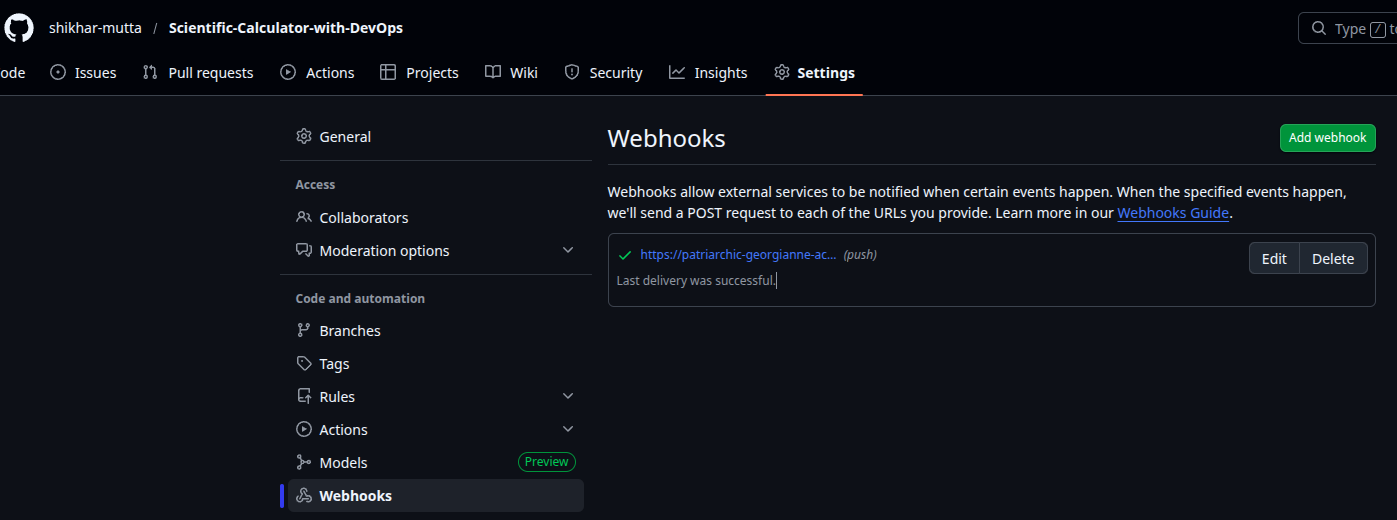
\includegraphics[width=\linewidth]{imgs/Github Webhook.png}
\caption{Webhook at git project setting}
\end{subfigure}
\hfill
\begin{subfigure}{0.45\textwidth}
\centering
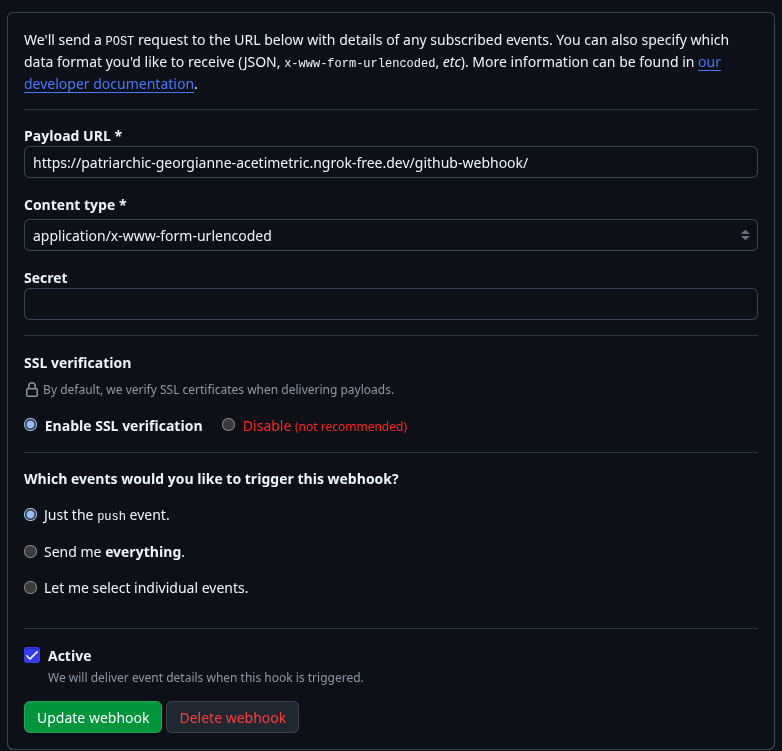
\includegraphics[width=\linewidth]{imgs/Github Webhook 1.png}
\caption{Webhook Configuration}
\end{subfigure}

\caption{GitHub Push Webhook}
\end{figure}

\begin{figure}[H]
\centering
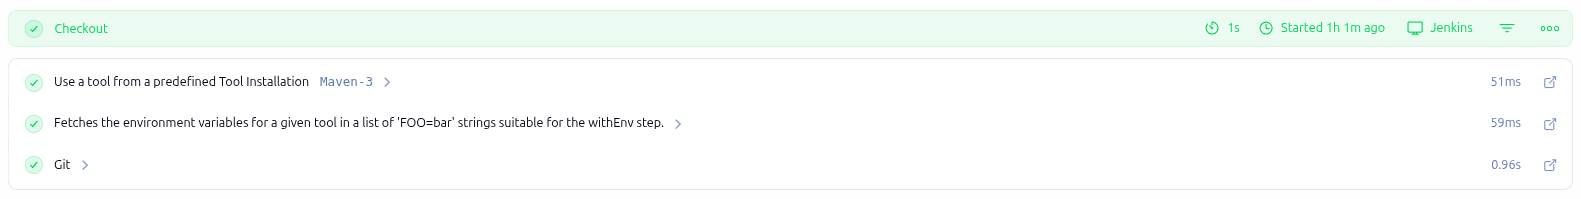
\includegraphics[width=1\textwidth]{imgs/Checkout.png}
\caption{Jenkins Checkout Stage}
\end{figure}

\subsection{Stage 2: Build}
\begin{verbatim}
stage('Build') {
    steps {
        script {
            try {
                sh 'mvn clean compile -q'
            } catch (Exception e) {
                currentBuild.description =
                  'Failed Stage: Build\nReason: Maven compilation failed.'
                throw e
            }
        }
    }
}
\end{verbatim}
\texttt{mvn clean compile -q} wipes previous build output and compiles all Java source files. The \texttt{-q} (quiet) flag suppresses verbose Maven output. Fails fast on syntax errors, preventing wasteful downstream steps from executing.

\begin{figure}[H]
\centering
% \fbox{\rule{0pt}{1.5in}\rule{4in}{0pt}}
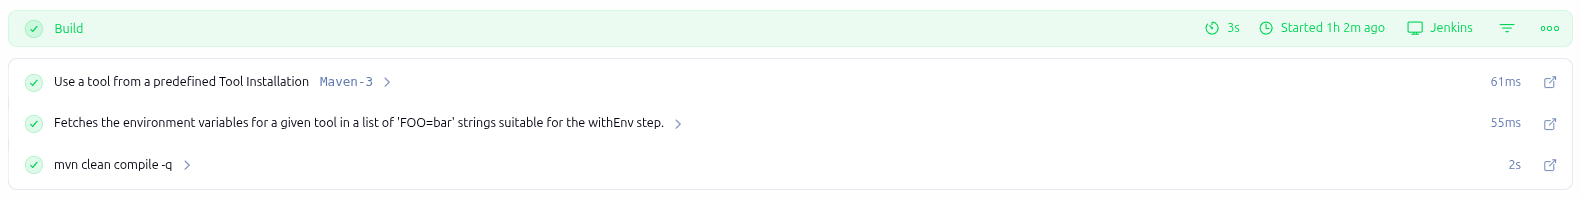
\includegraphics[width=1\textwidth]{imgs/Build.png}
\caption{Jenkins Console Output showing successful Maven Compilation}
\end{figure}

\subsection{Stage 3: Test}
\begin{verbatim}
stage('Test') {
    steps {
        script {
            try {
                sh 'mvn test'
            } catch (Exception e) {
                currentBuild.description =
                  'Failed Stage: Test\n' +
                  'Reason: One or more JUnit tests failed.'
                throw e
            }
        }
    }
}
\end{verbatim}
Runs the full JUnit 5 suite (37 tests) via Maven Surefire plugin. Tests cover all 8 operations including boundary cases and exception scenarios. Any failure marks the build as FAILURE and prevents broken code from being containerised and deployed.

\begin{figure}[H]
\centering
% \fbox{\rule{0pt}{1.5in}\rule{4in}{0pt}}
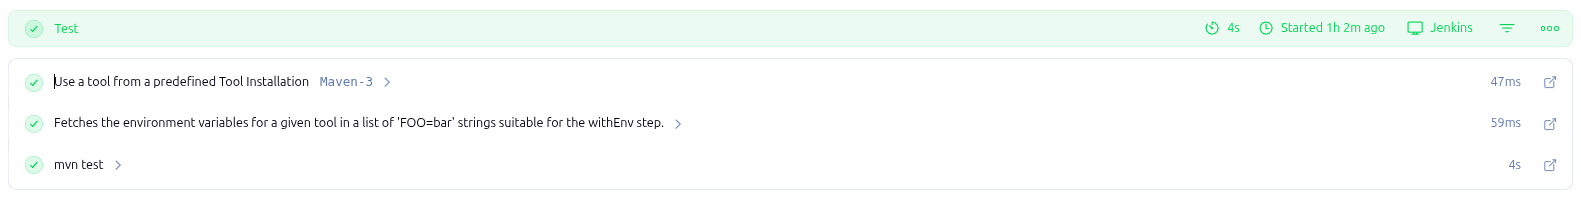
\includegraphics[width=1\textwidth]{imgs/test.png}
\caption{Jenkins Console Output displaying JUnit execution}
\end{figure}

\subsection{Stage 4: Package}
\begin{verbatim}
stage('Package') {
    steps {
        script {
            try {
                sh 'mvn package -DskipTests -q'
            } catch (Exception e) {
                currentBuild.description =
                  'Failed Stage: Package\n' +
                  'Reason: Failed to package the JAR file.'
                throw e
            }
        }
    }
}
\end{verbatim}
\begin{sloppypar}
The compiled classes are bundled into a runnable JAR (\texttt{scientific-calculator-}\allowbreak\texttt{1.0-SNAPSHOT.jar}) within the \texttt{target/} directory. Tests are skipped (\texttt{-DskipTests}) since they have already passed in Stage 3. This JAR is then copied into the Docker image during the next stage.
\end{sloppypar}

\begin{figure}[H]
\centering
% \fbox{\rule{0pt}{1.5in}\rule{4in}{0pt}}
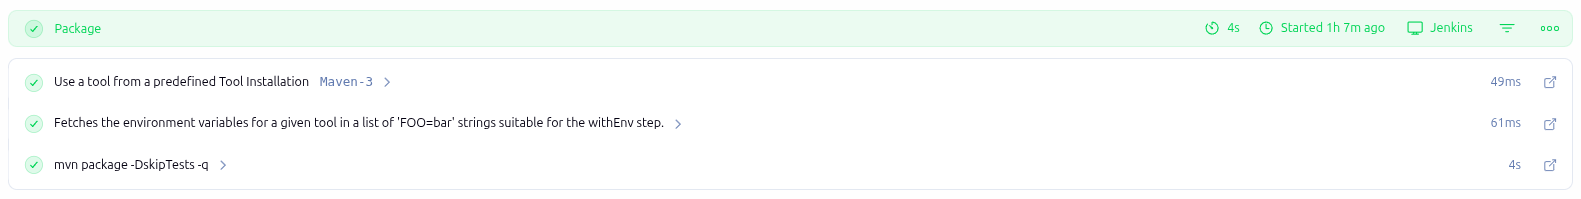
\includegraphics[width=1\textwidth]{imgs/Package.png}
\caption{Jenkins Console Output showing Maven JAR packaging}
\end{figure}

\subsection{Stage 5: Docker Build}
\begin{verbatim}
stage('Docker Build') {
    options {
        timeout(time: 15, unit: 'MINUTES')  // Kill stage if Docker hangs
    }
    steps {
        script {
            try {
                // Verify daemon reachable
                sh 'docker info > /dev/null 2>&1'         
                sh "docker build -t ${DOCKER_IMAGE}:${DOCKER_TAG} ."
            } catch (Exception e) {
                currentBuild.description =
                  'Failed Stage: Docker Build\n' + 
                  'Reason: Docker image build failed.'
                throw e
            }
        }
    }
}
\end{verbatim}
A 15-minute timeout guards against Docker daemon hangs. The pre-check \texttt{docker info} verifies the daemon is responsive. A 3-stage Dockerfile is used:
\begin{itemize}
    \item \textbf{Stage 1:} Maven builder --- downloads dependencies, compiles and packages the JAR
    \item \textbf{Stage 2:} \texttt{jlink} --- creates a custom minimal JRE including only the \texttt{java.base}, \texttt{java.logging}, and \texttt{java.desktop} modules (17.9 MB layer)
    \item \textbf{Stage 3:} Alpine 3.19.9 (3.26 MB base) + custom JRE + JAR (4.18 KB) --- final compressed image \textbf{21.17 MB}
\end{itemize}

\begin{figure}[H]
\centering
% \fbox{\rule{0pt}{1.5in}\rule{4in}{0pt}}
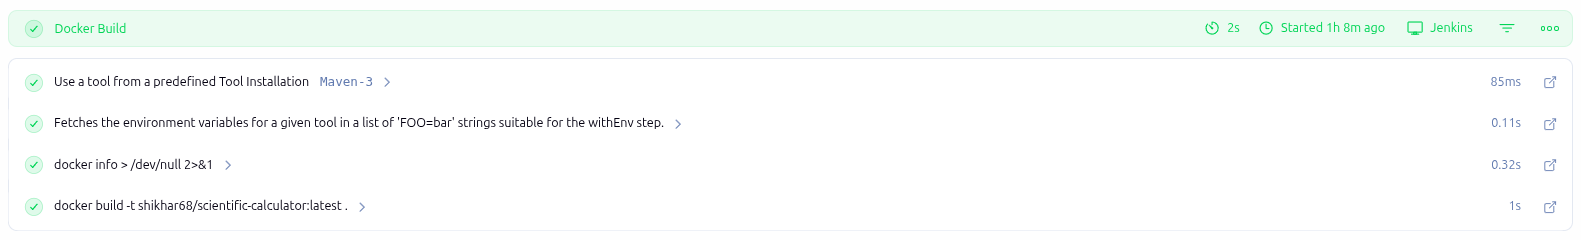
\includegraphics[width=1\textwidth]{imgs/Docker Build.png}
\caption{Jenkins Console Output showing Docker image build and layer caching}
\end{figure}

\subsection{Stage 6: Docker Push}
\begin{verbatim}
stage('Docker Push') {
    steps {
        script {
            try {
                withCredentials([usernamePassword(
                    credentialsId: 'docker-hub-credentials',
                    usernameVariable: 'DOCKER_USER',
                    passwordVariable: 'DOCKER_PASS'
                )]) {
                    sh "echo $DOCKER_PASS | docker login " +
                       "-u $DOCKER_USER --password-stdin"
                    sh "docker push ${DOCKER_IMAGE}:${DOCKER_TAG}"
                    sh 'docker logout'
                }
            } catch (Exception e) { ... }
        }
    }
}
\end{verbatim}
\begin{sloppypar}
Docker Hub credentials are stored in Jenkins Credential Manager (ID: \texttt{docker-hub-}\allowbreak\texttt{credentials}) and never appear in plain text. The password is passed via \texttt{--password-stdin} to avoid shell history exposure. \texttt{docker logout} clears credentials from the Jenkins agent after the push.
\end{sloppypar}

\begin{figure}[H]
\centering
% \fbox{\rule{0pt}{1.5in}\rule{4in}{0pt}}
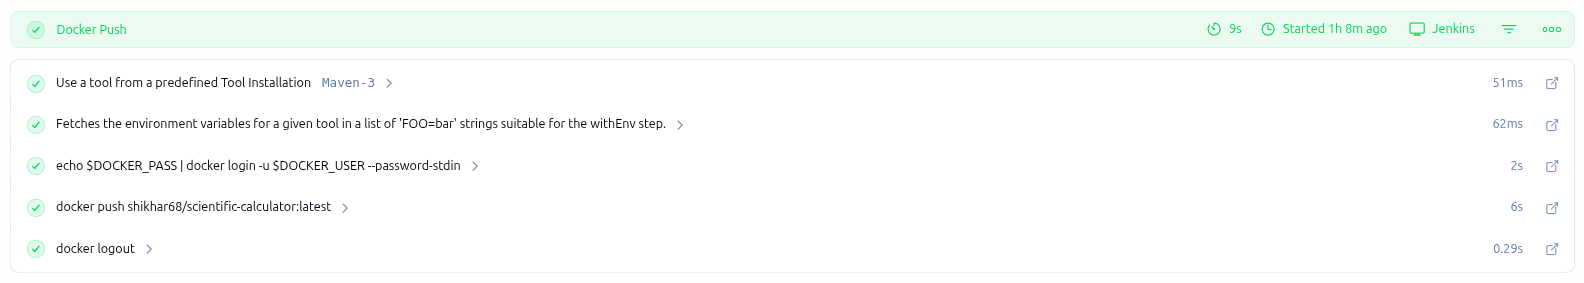
\includegraphics[width=1\textwidth]{imgs/Docker Push.png}
\caption{Jenkins Console Output showing Docker image push to DockerHub}
\end{figure}

\subsection{Stage 7: Deploy with Ansible}
\begin{verbatim}
stage('Deploy - Ansible') {
    steps {
        script {
            try {
                sh 'ansible-playbook -i inventory.ini deploy.yml'
            } catch (Exception e) {
                currentBuild.description =
                  'Failed Stage: Deploy\nReason: Ansible deployment failed.'
                throw e
            }
        }
    }
}
\end{verbatim}
\begin{sloppypar}
The Ansible playbook (\texttt{deploy.yml}) executes 6 tasks on localhost via \texttt{ansible\_connection=local}:
\end{sloppypar}
\begin{itemize}
    \item {[1]} Log the old container status (ID, Image, uptime) before update
    \item {[2]} Pull latest image from DockerHub (\texttt{docker pull})
    \item {[3]} Force-remove the existing container (\texttt{docker rm -f})
    \item {[4]} Start the new container: \texttt{docker run -d -i --restart unless-stopped} (\texttt{-i} keeps stdin open since the app is CLI-driven)
    \item {[5]} Verify the new container is running (\texttt{docker ps})
    \item {[6]} Print new container short ID for confirmation
\end{itemize}

\begin{figure}[H]
\centering
% \fbox{\rule{0pt}{1.5in}\rule{4in}{0pt}}
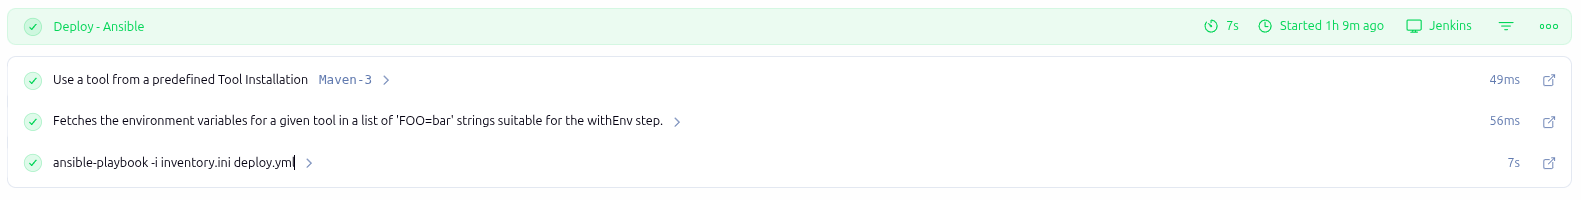
\includegraphics[width=1\textwidth]{imgs/Docker Ansible.png}
\caption{Jenkins Console Output showing Ansible playbook deployment execution}
\end{figure}

\subsection{Post --- Notifications \& Cleanup}
\begin{verbatim}
post {
    success {
        mail to: 'shikharmutta67@gmail.com',
             subject: "SUCCESS: Scientific Calculator Pipeline " +
                      "- Build #${env.BUILD_NUMBER}",
             body: "Pipeline completed successfully..."
    }
    failure {
        script {
            def info = currentBuild.description ?: 
                       'Failed Stage: SCM Checkout...'
            mail to: 'shikharmutta67@gmail.com',
                 subject: "FAILURE: Pipeline - Build " +
                          "#${env.BUILD_NUMBER}",
                 body: "Pipeline failed.\n\n${info}\n\n" +
                       "Console: ${env.BUILD_URL}console"
        }
    }
    always {
        sh 'docker image prune -f || true'   // Clean dangling images
    }
}
\end{verbatim}
\begin{figure}[H]
\centering
% \fbox{\rule{0pt}{1.5in}\rule{4in}{0pt}}
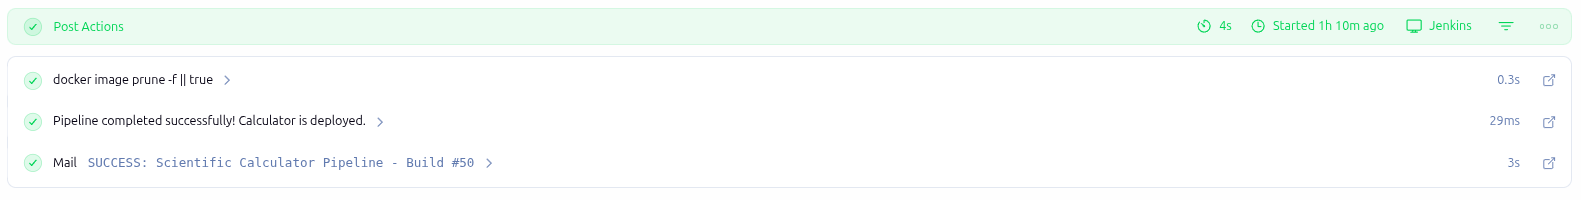
\includegraphics[width=1\textwidth]{imgs/Post Action.png}
\caption{Jenkins Console Output showing post-build actions and email notifications}
\end{figure}

Success and failure emails are sent via Jenkins Mailer plugin. Failure emails include the exact stage name and reason captured by each catch block. Dangling Docker images (intermediate build layers) are always pruned to conserve disk space.


\newpage

\section{Test Results \& Observations}
All 37 JUnit 5 unit tests pass consistently across every pipeline run. Tests cover both happy-path and error/exception scenarios for all 8 operations. Maven Surefire plugin reports: Tests run: 37, Failures: 0, Errors: 0, Skipped: 0

\begin{table}[H]
\centering
\begin{tabular}{|l|c|p{5.5cm}|c|}
\hline
\textbf{Test Group} & \textbf{Tests} & \textbf{What is Tested} & \textbf{Result} \\
\hline
Addition       & 4  & Positive, negative, zero, decimal inputs                                    & $\checkmark$ PASS \\
\hline
Subtraction    & 4  & Positive result, negative result, zero, same numbers                        & $\checkmark$ PASS \\
\hline
Multiplication & 4  & Positive, by zero, two negatives, mixed signs                               & $\checkmark$ PASS \\
\hline
Division       & 4  & Positive, negative, zero numerator, divide-by-zero throws                   & $\checkmark$ PASS \\
\hline
Power          & 5  & Pos/neg/zero/fractional exponent, base zero                                 & $\checkmark$ PASS \\
\hline
Square Root    & 4  & Positive, zero, decimal ($\sqrt{2}$), negative input throws                 & $\checkmark$ PASS \\
\hline
Natural Log    & 5  & $\ln(1)=0$, $\ln(e)=1$, $\ln(10)$, $\ln(0)$ throws, $\ln(-x)$ throws       & $\checkmark$ PASS \\
\hline
Factorial      & 7  & $0!$, $1!$, $5!$, $10!$, $20!$, negative throws, $n>20$ throws              & $\checkmark$ PASS \\
\hline
\textbf{TOTAL} & \textbf{37} & ---                                                                  & $\checkmark$ \textbf{ALL PASS} \\
\hline
\end{tabular}
\caption{Detailed Breakdown of JUnit Test Execution}
\end{table}

\textbf{Key Observations:}
\begin{itemize}
    \item \textbf{Exception coverage:} We utilize \texttt{assertThrows} (e.g., \texttt{IllegalArgumentException}\allowbreak\texttt{.class}) to verify correct error handling for invalid inputs (such as divide-by-zero, square root of negative, logarithm of non-positive, and factorial overflow).
    \item \textbf{Floating-point precision:} All double comparisons use a delta of $1\mathrm{e}{-9}$ to handle IEEE 754 floating-point rounding correctly.
    \item \textbf{Stage separation:} Tests are a separate pipeline stage from Build --- a test failure gives clear feedback without rerequiring recompilation.
    \item \textbf{Performance:} The test stage completes in approximately 2--4 seconds due to pure unit tests with no I/O or network calls.
\end{itemize}

\begin{figure}[H]
\centering
% \fbox{\rule{0pt}{1.5in}\rule{4in}{0pt}}
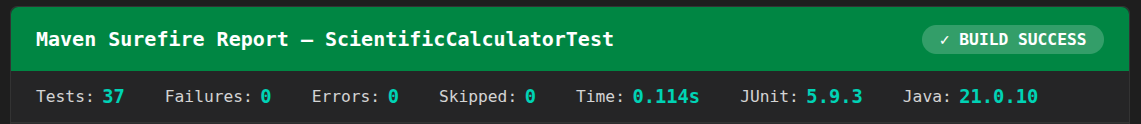
\includegraphics[width=1\textwidth]{imgs/Test Cases.png}
\caption{Detailed Output of the Test Cases or Surefire Reports}
\end{figure}

\newpage

\section{System Architecture \& Resource Pruning}

Keeping the Docker image small and the build environment clean are critical for a sustainable CI/CD pipeline. This project employs two complementary strategies: a multi-stage Dockerfile with \texttt{jlink} to minimise the production image, and automated post-build cleanup to reclaim disk space on the Jenkins agent.

\subsection{Multi-Stage Dockerfile with jlink}
The Dockerfile uses three distinct stages to produce a minimal, production-ready container image:

\begin{enumerate}
    \item \begin{sloppypar}\textbf{Stage 1 --- Maven Builder} (\texttt{maven:3.9-eclipse-temurin-17}): Dependencies are downloaded and cached via \texttt{mvn dependency:go-offline}. The application is then compiled and packaged into a runnable JAR (\texttt{scientific\-calculator\-1.0\-SNAPSHOT.jar}) using \texttt{mvn clean package -DskipTests -o -q}. Separating the dependency download from the build step enables Docker layer caching --- subsequent builds skip the download if \texttt{pom.xml} has not changed.\end{sloppypar}

    \item \begin{sloppypar}\textbf{Stage 2 --- Custom JRE via jlink} (\texttt{eclipse-temurin:17-jdk-alpine}): The Alpine JDK variant is used so that the output is \texttt{musl}-compatible. \texttt{jlink} creates a stripped-down JRE containing only the modules the application requires:\end{sloppypar}
    \begin{verbatim}
    jlink --add-modules java.base,java.logging \
          --strip-debug --no-man-pages \
          --no-header-files --compress=2 \
          --output /custom-jre
    \end{verbatim}
    Flags such as \texttt{--strip-debug}, \texttt{--no-man-pages}, and \texttt{--compress=2} further reduce the JRE size from $\sim$300\,MB (full JDK) down to $\sim$18\,MB.

    \item \textbf{Stage 3 --- Alpine Runtime} (\texttt{alpine:3.19}): The final image copies only the custom JRE and the application JAR onto a bare Alpine 3.19 base (3.26\,MB). A non-root user (\texttt{appuser}) is created for security, and the entrypoint is set to \texttt{java -jar app.jar}.
\end{enumerate}

\noindent The resulting production image is approximately \textbf{21\,MB} --- a $\sim$96\% reduction compared to a naive single-stage build using the full JDK image ($\sim$500\,MB).

\begin{table}[H]
\centering
\begin{tabular}{|l|r|l|}
\hline
\textbf{Layer} & \textbf{Size} & \textbf{Purpose} \\
\hline
Alpine 3.19 base  & 3.26\,MB  & Minimal OS (musl libc, BusyBox) \\
\hline
Custom JRE (jlink) & $\sim$17.9\,MB & java.base + java.logging only \\
\hline
Application JAR    & 4.18\,KB  & Compiled calculator classes \\
\hline
\textbf{Total}     & \textbf{$\sim$21\,MB} & \textbf{Final compressed image} \\
\hline
\end{tabular}
\caption{Docker image layer breakdown}
\end{table}

\subsection{Post-Build Disk Cleanup}
Every pipeline run --- whether it succeeds or fails --- triggers a post-build action in the \texttt{always} block of the Jenkinsfile:
\begin{verbatim}
post {
    always {
        sh 'docker image prune -f || true'
    }
}
\end{verbatim}
\texttt{docker image prune -f} removes all \textit{dangling} images (untagged intermediate layers left behind by multi-stage builds). The \texttt{|| true} suffix ensures the pipeline does not fail if there are no images to prune. Over multiple builds, this prevents unbounded disk consumption on the Jenkins agent.

\begin{figure}[H]
\centering
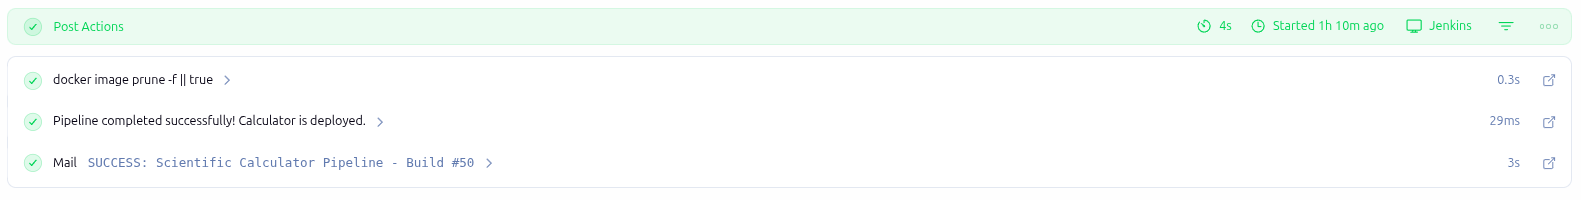
\includegraphics[width=1\textwidth]{imgs/Post Action.png}
% \fbox{\rule{0pt}{1.5in}\rule{4in}{0pt}}
\caption{Jenkins post-build actions: Docker image pruning and email notifications}
\end{figure}

\newpage

\section{Application Output}
Because this is a command-line interface application executed securely inside a microservice container, it is provisioned completely detached from the local machine's host OS vulnerabilities. End users access it via standard interactive TTY hooks.

\begin{figure}[H]
\centering
% \fbox{\rule{0pt}{2in}\rule{4in}{0pt}}
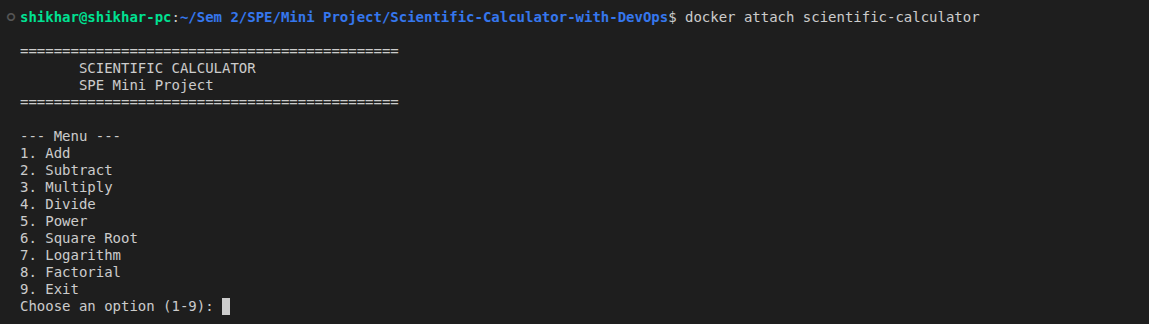
\includegraphics[width=1\textwidth]{imgs/docker attach.png}
\caption{Execution of \texttt{docker attach scientific-calculator} showing the calculator UI}
\end{figure}

\begin{figure}[H]
\centering
% \fbox{\rule{0pt}{2in}\rule{4in}{0pt}}
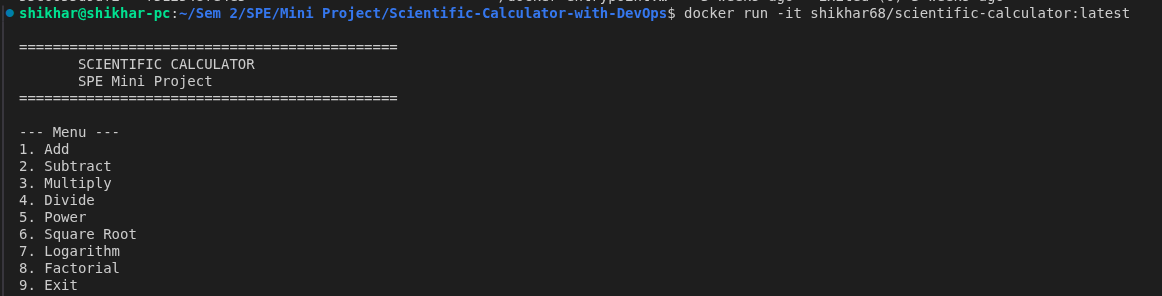
\includegraphics[width=1\textwidth]{imgs/docker run.png}
\caption{Execution of \texttt{docker run -it shikhar68/scientific-calculator:latest} showing the calculator UI}
\end{figure}

\begin{figure}[H]
\centering
\begin{subfigure}{0.32\textwidth}
  \centering
  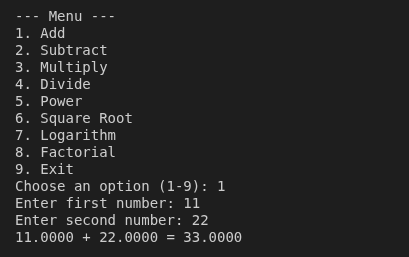
\includegraphics[width=\linewidth]{imgs/O1.png}
\end{subfigure}\hfill
\begin{subfigure}{0.32\textwidth}
  \centering
  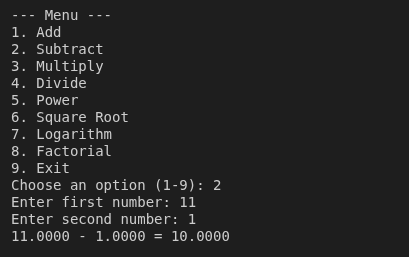
\includegraphics[width=\linewidth]{imgs/O2.png}
\end{subfigure}\hfill
\begin{subfigure}{0.32\textwidth}
  \centering
  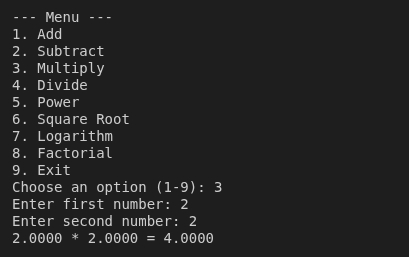
\includegraphics[width=\linewidth]{imgs/O3.png}
\end{subfigure}

\vspace{0.3cm}
\begin{subfigure}{0.32\textwidth}
  \centering
  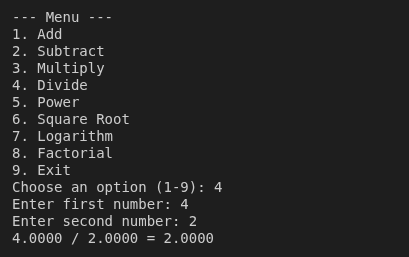
\includegraphics[width=\linewidth]{imgs/O4.png}
\end{subfigure}\hfill
\begin{subfigure}{0.32\textwidth}
  \centering
  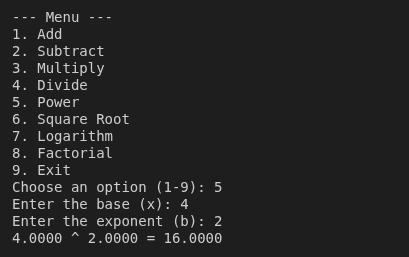
\includegraphics[width=\linewidth]{imgs/O5.png}
\end{subfigure}\hfill
\begin{subfigure}{0.32\textwidth}
  \centering
  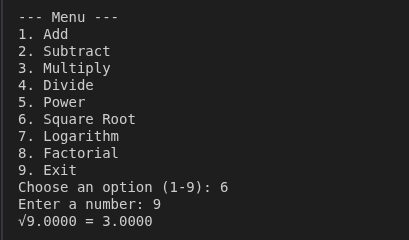
\includegraphics[width=\linewidth]{imgs/O6.png}
\end{subfigure}

\vspace{0.3cm}
\begin{subfigure}{0.32\textwidth}
  \centering
  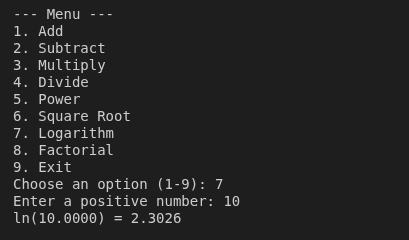
\includegraphics[width=\linewidth]{imgs/O7.png}
\end{subfigure}\hfill
\begin{subfigure}{0.32\textwidth}
  \centering
  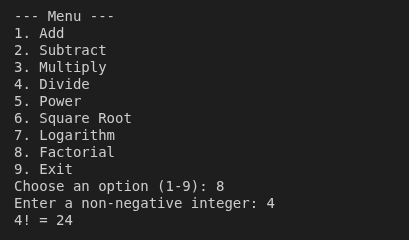
\includegraphics[width=\linewidth]{imgs/O8.png}
\end{subfigure}\hfill
\begin{subfigure}{0.32\textwidth}
  \centering
  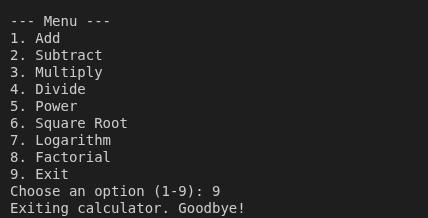
\includegraphics[width=\linewidth]{imgs/O9.png}
\end{subfigure}
\caption{Mathematical operations returning accurate answers inside the terminal}
\end{figure}

\end{document}
